\documentclass{article}

% Encodings, page setup, paragraph formatting, font
\usepackage[top=0.9in, bottom=1in, left=1.5in, right=1.5in]{geometry}
\usepackage[utf8]{inputenc}
\usepackage[icelandic]{babel}
\usepackage[T1]{fontenc}
\usepackage[sc]{mathpazo}
\usepackage[parfill]{parskip}

% Tables and lists
\usepackage{booktabs,tabularx}
\usepackage{multirow}
\usepackage{enumerate}

% Math
\usepackage{amsmath, amsfonts, amssymb, amsthm}

% Graphics
\usepackage{graphicx}
\usepackage{tikz}

% Code environment
\usepackage{minted}

% Hyperlinks and related
\usepackage[bookmarks=true,colorlinks=true,pdfauthor={Magnús Pálsson},linkcolor=blue,urlcolor=blue]{hyperref}

% Minted configuration
\usemintedstyle{default}
\renewcommand{\theFancyVerbLine}{\sffamily \arabic{FancyVerbLine}}
\floatstyle{plaintop}
\newfloat{program}{thp}{lop}
\floatname{program}{Forrit}

% macros
\newcommand\norm[1]{\left\lVert#1\right\rVert}

% Meta information
\date{}
\author{Magnús Pálsson}
% Hyphenation
\hyphenpenalty=5000
% Page and section numbering
\setcounter{secnumdepth}{-1} 
\pagenumbering{gobble}
\usepackage{bm}


\title{Seismology \\ - \\ \large Homework 1}
\author{Magnús Pálsson}
\begin{document}
\maketitle

\section*{Problem 1}
Assume that the horizontal components of the 2-D stress tensor are
\begin{equation*}
\boldsymbol{\tau} = 
    \begin{bmatrix}
        \tau_{xx} & \tau_{xy} \\
        \tau_{yx} & \tau_{yy}
    \end{bmatrix}
    =
    \begin{bmatrix}
        -30 & -20 \\
        -20 & -40
    \end{bmatrix}
    \text{MPa}
\end{equation*}

\textbf{(a)} Compute the normal and shear stresses on a fault that strikes 10° east of north.

\textbf{(b)} Compute the principal stresses, and give the azimuths (in degrees east of north) of the maximum and minimum compressional stress axes.

\subsection*{(a) Solution}
We have 
\begin{equation*}
    \hat{\mathbf{n}} = 
    \begin{bmatrix}
        \cos(10^{\circ}) \\
        -\sin(10^{\circ})
    \end{bmatrix}
    \approx 
    \begin{bmatrix}
        0.9848 \\
        -0.1736
    \end{bmatrix}
\end{equation*}
And 
\begin{equation*}
    \mathbf{t}(\hat{\mathbf{n}}) = \boldsymbol{\tau}\hat{\mathbf{n}} \approx
    \begin{bmatrix}
        -30 & -20 \\
        -20 & -40
    \end{bmatrix}
    \begin{bmatrix}
        0.9848 \\
        -0.1736
    \end{bmatrix}
    \approx
    \begin{bmatrix}
        -26.0713 \\
        -12.7502
    \end{bmatrix}
\end{equation*}
This gives us 
\begin{equation*}
    t_N = \mathbf{t}(\hat{\mathbf{n}}) \cdot \hat{\mathbf{n}} \approx 
    \begin{bmatrix}
        -26.0713 \\
        -12.7502
    \end{bmatrix}
    \cdot
    \begin{bmatrix}
        0.9848 \\
        -0.1736
    \end{bmatrix}
    \approx -23.4611
\end{equation*}
And 
\begin{equation*}
    t_S = \sqrt{\norm{\mathbf{t}(\hat{\mathbf{n}})}^2 - t_N^2} \approx 17.0837
\end{equation*}


\subsection*{(b) Solution}

To find the principal stresses we need the eigenvalues of $\boldsymbol{\tau}$. Using Python we find them to be $\lambda_1 = -55.6155$ and $\lambda_2 = -14.3845$. The associated eigenvectors are 
\begin{equation*}
    \mathbf{u}^{(1)} \approx
    \begin{bmatrix}
        0.6154 \\
        0.7882
    \end{bmatrix}
    , \quad \text{and} \quad
    \mathbf{u}^{(2)} \approx
    \begin{bmatrix}
        0.7882 \\
        -0.6154
    \end{bmatrix}
\end{equation*}

The azimuth in degrees east of north of the maximum compressional stress axis is 
\begin{equation*}
    \sin^{-1}\left( \frac{\mathbf{u}^{(1)}_x}{\norm{\mathbf{u}^{(1)}}} \right) \approx
    \sin^{-1}\left(\frac{0.6154}{1}\right) \approx 
    \sin^{-1}\left( 0.6154\right) = 37.9819^{\circ}
\end{equation*}
As for the minimum compressional stress axis it will be perpendicular to the maximum compressional stress axis and inspection reveals that the azimuth in degrees east of north is $37.9819^{\circ} + 90^{\circ} = 127.9819$
\pagebreak
\section*{Problem 3}
Consider two types of monochromatic plane waves propagating in the x direction in a uniform medium: 

\textbf{(a)} $P$ wave in which $u_x = A\sin(\omega t-kx)$,

\textbf{(b)} $S$ wave with displacements in the $y$ direction, i.e., $u_y = A\sin(\omega t-kx)$

For each case, derive expressions for the non-zero components of the stress tensor.

\subsection*{Solution (a)}

Of all the partial derivatives of $\mathbf{u}$, only the x derivative of the x component $\partial_x u_x = -kA\cos(\omega t-kx)$ is non-zero. We will avoid writing out the full expression to save space, writing the strain and stress in terms of $\partial_x u_x$. We get the strain tensor:

\begin{equation*}
    \mathbf{e} = 
    \begin{bmatrix}
        \partial_x u_x & \frac{1}{2}\partial_x u_x & \frac{1}{2}\partial_x u_x \\
        \frac{1}{2}\partial_x u_x & 0 & 0\\
        \frac{1}{2}\partial_x u_x & 0 & 0
    \end{bmatrix}
\end{equation*}

We see that $\text{tr}(\mathbf{e}) = \partial_x u_x$ so eqn. 2.30 from Shearer gives us the stress tensor:

\begin{equation*}
    \boldsymbol{\tau} = 
    \begin{bmatrix}
        (\lambda + 2\mu) \partial_x u_x & \mu \partial_x u_x & \mu \partial_x u_x\\
        \mu \partial_x u_x  & \lambda \partial_x u_x & 0 \\
        \mu \partial_x u_x & 0 & \lambda \partial_x u_x 
    \end{bmatrix}
    = \partial_x u_x 
    \begin{bmatrix}
        (\lambda + 2\mu) & \mu  & \mu \\
        \mu   & \lambda & 0 \\
        \mu  & 0 & \lambda 
    \end{bmatrix}
\end{equation*}

\subsection*{Solution (b)}

For the S wave, only the y component of $\mathbf{u}$ is non-zero and it only depends on x. Therefore, of the partial derivatives of the components of $\mathbf{u}$, only $\partial_xu_y = -kA\cos(\omega t-kx)$ is non-zero. This gives us the strain tensor:

\begin{equation*}
    \mathbf{e} = 
    \begin{bmatrix}
        0 & \frac{1}{2}\partial_x u_y & 0 \\
        \frac{1}{2}\partial_x u_y & 0 & 0\\
        0 & 0 & 0
    \end{bmatrix}
\end{equation*}

We see that $\text{tr}(\mathbf{e}) = 0$ so eqn. 2.30 from Shearer gives us the stress tensor:

\begin{equation*}
    \boldsymbol{\tau} = 
    \begin{bmatrix}
        0 & \mu\frac{1}{2}\partial_x u_y & 0 \\
        \mu\frac{1}{2}\partial_x u_y & 0 & 0\\
        0 & 0 & 0
    \end{bmatrix}
\end{equation*}
\pagebreak
\section*{Problem 4}
Show that the principal stress axes always coincide with the principal strain axes for isotropic media. In other words, show that if $\mathbf{x}$ is an eigenvector of $\mathbf{e}$, then it is also an eigenvector of $\boldsymbol{\tau}$.

\subsection*{Solution}

We use the relationship
\begin{equation*}
    \boldsymbol{\tau} = 
    \lambda \text{tr}(\mathbf{e})\mathbf{I} +
    2\mu \mathbf{e}
\end{equation*}
and the definition of eigenvectors/eigenvalues of a matrix, $\mathbf{ex} = a \mathbf{x}$, using $a$ rather than the more traditional $\lambda$ to avoid confusion. Note that the trace of a matrix is a scalar.
\begin{align*}
    \boldsymbol{\tau}\mathbf{x} &= (\lambda \text{tr}(\mathbf{e})\mathbf{I} + 2\mu \mathbf{e}) \mathbf{x} \\
    &= \lambda \text{tr}(\mathbf{e})\mathbf{I} \mathbf{x} + 
    2\mu \mathbf{e}\mathbf{x} \\
    &= \lambda \text{tr}(\mathbf{e})\mathbf{x} + 
    2\mu a \mathbf{x} \\
    &= (\lambda \text{tr}(\mathbf{e}) + 
    2\mu a) \mathbf{x} \\
    &= b \mathbf{x}
\end{align*}
So $\mathbf{x}$ is an eigenvector of $\boldsymbol{\tau}$ with the eigenvalue of $b = (\lambda \text{tr}(\mathbf{e}) + 2\mu a)$.\\

From eqn. 2.30 in the book we can calculate that $\text{tr}(\boldsymbol{\tau}) = 3\lambda\text{tr}(\mathbf{e}) + 2 \mu \text{tr}(\mathbf{e})$ meaning that 
\begin{equation*}
    \text{tr}(\mathbf{e}) = \frac{\text{tr}(\boldsymbol{\tau})}{3\lambda + 2\mu}
\end{equation*}

giving us the eiginvalue of $\boldsymbol{\tau}$, $b$ corresponding to the eigenvector $\mathbf{x}$

\begin{equation*}
    b = \frac{\lambda}{3\lambda + 2\mu} \text{tr}(\boldsymbol{\tau}) + 2\mu a
\end{equation*}

\pagebreak
\section*{Problem 7}
We use the code from the book as a guide and flesh out the following script

\inputminted{python}{P7script.py}

\pagebreak

The output images are as follows
\begin{figure*}[h]
    \centering
    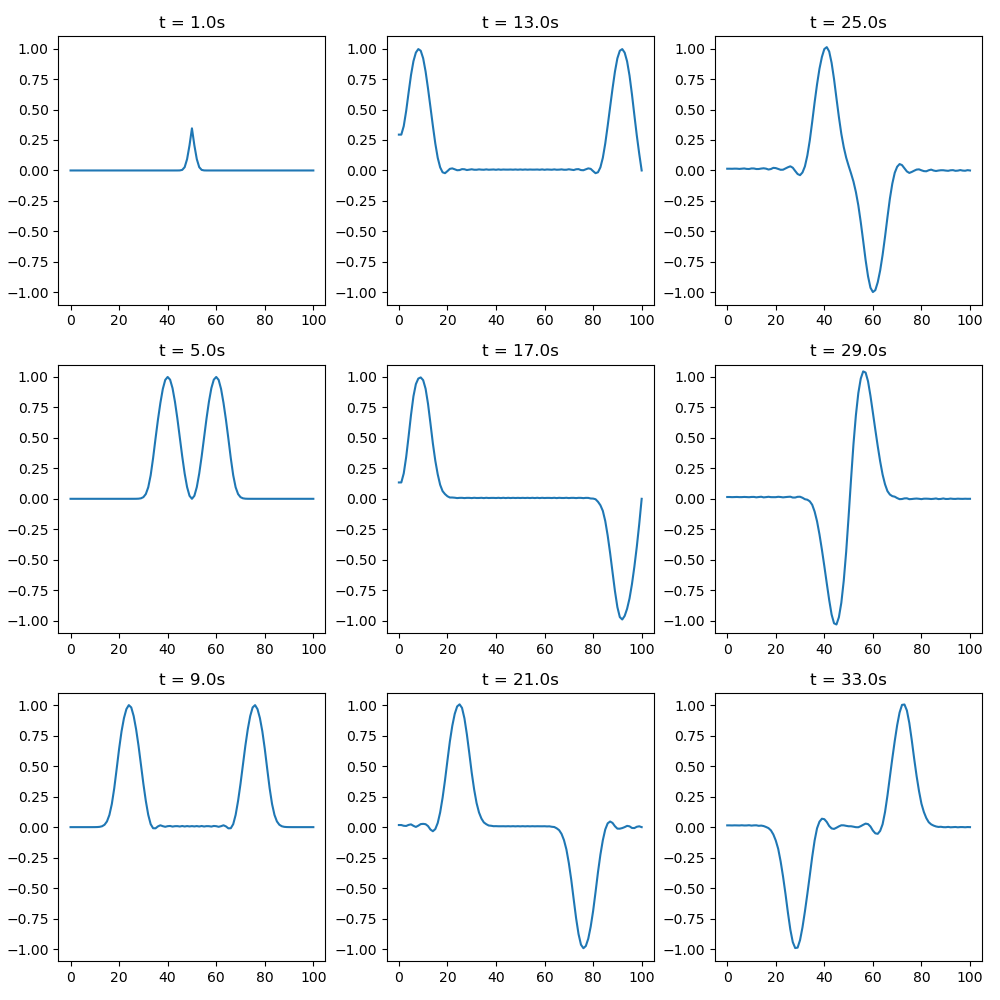
\includegraphics[scale=0.55]{figures/P7output}
\end{figure*}

We see that The pulse hitting the stress free boundary is reflected as is but the pulse hitting the fixed boundary has its displacement mirrored as it is reflected back. When the pulses meet they pass through each other.
\pagebreak
\section*{Problem 9}

Using values from the PREM model, compute values for the bulk modulus on both sides of 

\textbf{(a)} the core-mantle boundary (CMB)\\
\textbf{(b)} the inner-core boundary 

Express your answers in pascals.

\subsection*{Solution}

We start by deriving an equation for the bulk modulus in terms of the speed of P and S waves. From the given formulas we have:

\begin{equation*}
    \beta^2 = \frac{\mu}{\rho}, \quad \mu = \rho \beta^2
\end{equation*}
\begin{equation*}
    \alpha^2 = \frac{\lambda + 2 \mu}{\rho} = \frac{\lambda + 2 \rho \beta}{\rho}, \quad \lambda = \rho \alpha^2 - 2 \rho \beta^2
\end{equation*}

Now

\begin{equation*}
    \kappa = \lambda + \frac{2}{3} \mu = 
    \rho \alpha^2 - 2 \rho \beta^2 + \frac{2}{3} \rho \beta^2 = 
    \rho(\alpha^2 - \frac{4}{3} \beta^2)
\end{equation*}

Now that we have the equation, we need to think about units. To get the answer in Pa we have to transform the units in the table to SI units, this happens to be a factor of a 1000 for each parameter, resulting in a total factor of $10^{9}$. We can therefore calculate with the units in the table and get the answer in GPa.

We also note that S waves do not probagate in liquid so we can see the estimated boundaries in the table from that. Finally we can do the calculations

\subsection*{(a)}
\subsubsection*{Above the boundary}
\begin{equation*}
    5.57\times(13.72^2 - \frac{4}{3}\times 7.26^2) = 657 \; \text{GPa}
\end{equation*}

\subsubsection*{Below the boundary}
\begin{equation*}
    9.90\times(8.06^2 - \frac{4}{3}\times 0^2) = 643 \; \text{GPa}
\end{equation*}


\subsection*{(b)}
\subsubsection*{Above the boundary}
\begin{equation*}
    12.17\times(10.36^2 - \frac{4}{3}\times 0^2) = 1306 \; \text{GPa}
\end{equation*}

\subsubsection*{Below the boundary}
\begin{equation*}
    12.76\times(11.03^2 - \frac{4}{3}\times 3.50^2) = 1344 \; \text{GPa}
\end{equation*}
\end{document}